\documentclass[12pt,aspectratio=43]{beamer}
\usepackage{tikz}
\usetheme{Boadilla}
\setbeamertemplate{navigation symbols}{}
\title{Message passing: experiments and bounds}
\subtitle{Generated interaction study}
\author{Research group}
\date{}
\year=2026\month=11\day=5
\newcommand{\fuzzlayerA}[1]{\textbf{#1}}
\newcommand{\fuzzterm}[1]{\fuzzlayerA{#1}}
\newcommand{\fuzzpair}[2]{\fuzzterm{#1}: #2}
\newcommand{\fuzzunit}{ms}
\let\fuzzoriginalunit\fuzzunit
\newcommand{\fuzzcoefficient}{1}
\newcommand{\fuzzscale}[2][\fuzzcoefficient]{#1\,#2}
\definecolor{fuzzpaint}{RGB}{255,0,255}
\definecolor{fuzzsecond}{RGB}{18,137,67}
\tikzset{fuzzvertex/.style={draw,rounded corners=1pt,fill=blue!10,inner sep=1pt,minimum width=.35cm,minimum height=.25cm}}
\begin{document}
\section{Message passing}
\begin{frame}[t,shrink=5]{Message passing}{Composed dependencies}
\fuzzpair{Experiment}{Timing: 12\fuzzunit; estimate $\fuzzscale{x}+\fuzzscale[2]{y}$.}\par
{\renewcommand{\fuzzunit}{cycles}\let\fuzzterm\textrm\fuzzpair{LocalScope}{Timing: 7\fuzzunit.}\par}
\fuzzpair{RestoredScope}{Timing: 11\fuzzunit.}\par
\begin{columns}[onlytextwidth,b]
\begin{column}{0.38\textwidth}
\begin{enumerate}
\item<1-> {\scriptsize\color{black}\centering
\textrm{Intermediate results carry} both a numerical estimate and an explicit dependency set.  The estimate is $\frac{a+b}{1+c}$.\par}
\item<2-> \begin{description}
\item<1->[Stage 1] \begin{itemize}
\item<1-> 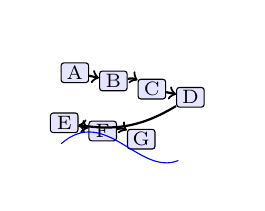
\begin{tikzpicture}[font=\scriptsize]
\begin{scope}[scale=1,rotate=-12]
\clip (-.4,-1) rectangle (2.000,.5);

\node[fuzzvertex] (g6n0) at (0.000,0) {A};
\node[fuzzvertex] (g6n1) at (0.500,0) {B};
\node[fuzzvertex] (g6n2) at (1.000,0) {C};
\node[fuzzvertex] (g6n3) at (1.500,0) {D};
\node[fuzzvertex] (g6n4) at (0.000,-0.65) {E};
\node[fuzzvertex] (g6n5) at (0.500,-0.65) {F};
\node[fuzzvertex] (g6n6) at (1.000,-0.65) {G};
\begin{scope}[xshift=.5pt,yshift=-.5pt]
\draw<1->[->,thick] (g6n0) -- (g6n1);
\draw<1->[->,thick] (g6n1) to[bend left=20] (g6n2);
\draw<1->[->,thick] (g6n2) -- (g6n3);
\draw<1->[->,thick] (g6n3) to[bend left=20] (g6n4);
\draw<1->[->,thick] (g6n4) -- (g6n5);
\draw<1->[->,thick] (g6n5) to[bend left=20] (g6n6);
\draw[blue] (0,-.9) .. controls (0.450,-.3) and (1.050,-1.1) .. (1.500,-.8);
\end{scope}
\end{scope}
\end{tikzpicture}
\end{itemize}
\item<2->[Stage 2] \begin{description}
\item<1->[Stage 1] \begin{tabular}{lrr}Method&Cost&Error\\\hline
Global0&19&26\\
Cached1&17&16\\
\end{tabular}
\end{description}
\end{description}
\end{enumerate}
\end{column}
\begin{column}{0.58\textwidth}
\begin{itemize}
\item<1-> \begin{columns}[onlytextwidth,t]
\begin{column}{0.62\textwidth}
\begin{exampleblock}{Message passing}
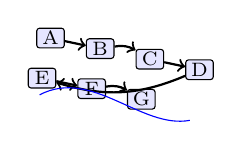
\begin{tikzpicture}[font=\scriptsize]
\begin{scope}[scale=0.8,rotate=-12]


\node[fuzzvertex] (g12n0) at (0.000,0) {A};
\node[fuzzvertex] (g12n1) at (0.806,0) {B};
\node[fuzzvertex] (g12n2) at (1.612,0) {C};
\node[fuzzvertex] (g12n3) at (2.418,0) {D};
\node[fuzzvertex] (g12n4) at (0.000,-0.65) {E};
\node[fuzzvertex] (g12n5) at (0.806,-0.65) {F};
\node[fuzzvertex] (g12n6) at (1.612,-0.65) {G};
\begin{scope}[xshift=.5pt,yshift=-.5pt]
\draw<1->[->,thick] (g12n0) -- (g12n1);
\draw<1->[->,thick] (g12n1) to[bend left=20] (g12n2);
\draw<1->[->,thick] (g12n2) -- (g12n3);
\draw<1->[->,thick] (g12n3) to[bend left=20] (g12n4);
\draw<1->[->,thick] (g12n4) -- (g12n5);
\draw<1->[->,thick] (g12n5) to[bend left=20] (g12n6);
\draw[blue] (0,-.9) .. controls (0.725,-.3) and (1.693,-1.1) .. (2.418,-.8);
\end{scope}
\end{scope}
\end{tikzpicture}
\end{exampleblock}
\end{column}
\begin{column}{0.34\textwidth}
\visible<1-2>{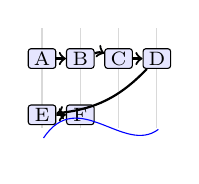
\begin{tikzpicture}[font=\scriptsize]
\begin{scope}[scale=1.1,rotate=0]

\foreach \x in {0,1,2,3} {\draw[gray!30] (\x*0.442,-.8)--(\x*0.442,.35);}
\node[fuzzvertex] (g14n0) at (0.000,0) {A};
\node[fuzzvertex] (g14n1) at (0.442,0) {B};
\node[fuzzvertex] (g14n2) at (0.884,0) {C};
\node[fuzzvertex] (g14n3) at (1.326,0) {D};
\node[fuzzvertex] (g14n4) at (0.000,-0.65) {E};
\node[fuzzvertex] (g14n5) at (0.442,-0.65) {F};
\begin{scope}[xshift=.5pt,yshift=-.5pt]
\draw<1->[->,thick] (g14n0) -- (g14n1);
\draw<1->[->,thick] (g14n1) to[bend left=20] (g14n2);
\draw<1->[->,thick] (g14n2) -- (g14n3);
\draw<1->[->,thick] (g14n3) to[bend left=20] (g14n4);
\draw<1->[->,thick] (g14n4) -- (g14n5);
\draw[blue] (0,-.9) .. controls (0.398,-.3) and (0.928,-1.1) .. (1.326,-.8);
\end{scope}
\end{scope}
\end{tikzpicture}}
\end{column}
\end{columns}
\item<2-> \begin{block}{Iterative refinement}
\[\begin{pmatrix}a&b\\c&d\end{pmatrix}\begin{pmatrix}x\\y\end{pmatrix}\]
\end{block}
\end{itemize}
\end{column}
\end{columns}
\par 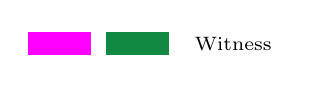
\begin{tikzpicture}[font=\scriptsize]
\fill<2-3>[fuzzpaint] (0,0) rectangle (.8,.3);
\fill<3->[fuzzsecond] (1,0) rectangle (1.8,.3);
\node[anchor=west] at (2,0.15) {Witness};
\end{tikzpicture}
\only<4>{}
\end{frame}
\renewcommand{\fuzzunit}{us}
\renewcommand{\fuzzcoefficient}{2}
\renewcommand{\fuzzterm}[1]{{\textit{#1}}}
\section{Cache invalidation}
\begin{frame}[t]{Cache invalidation}
\fuzzpair{MacroStageB}{Timing: 12\fuzzunit, retained: 9\fuzzoriginalunit.}\par
{\renewcommand{\fuzzunit}{local}\fuzzpair{FrameLocal}{Timing: 5\fuzzunit.}\par}
\fuzzpair{FrameRestored}{Timing: 8\fuzzunit; estimate $\fuzzscale{x}$.}\par
\begin{columns}[T]\begin{column}{.46\textwidth}The next pass must preserve the boundary conditions while revisiting dependent values.\end{column}\begin{column}{.46\textwidth}\begin{itemize}\item Input state\item Updated state\end{itemize}\end{column}\end{columns}
\end{frame}
\renewcommand{\fuzzunit}{min}
\renewcommand{\fuzzcoefficient}{3}
\renewcommand{\fuzzterm}[1]{{\textbf{#1}}}
\section{Message passing}
\begin{frame}[t]{Constraint propagation}
\fuzzpair{MacroStageC}{Timing: 12\fuzzunit, retained: 9\fuzzoriginalunit.}\par
{\renewcommand{\fuzzunit}{local}\fuzzpair{FrameLocal}{Timing: 5\fuzzunit.}\par}
\fuzzpair{FrameRestored}{Timing: 8\fuzzunit; estimate $\fuzzscale{x}$.}\par
\begin{block}{Follow-up}\fuzzterm{A revised value} depends on the preceding frame.\end{block}
\[r_{k+1}=r_k-\alpha d_k\]
\end{frame}
\renewcommand{\fuzzunit}{us}
\renewcommand{\fuzzcoefficient}{4}
\renewcommand{\fuzzterm}[1]{{\textbf{#1}}}
\section{Geometric uncertainty}
\begin{frame}[t]{Geometric uncertainty}
\fuzzpair{MacroStageD}{Timing: 12\fuzzunit, retained: 9\fuzzoriginalunit.}\par
{\renewcommand{\fuzzunit}{local}\fuzzpair{FrameLocal}{Timing: 5\fuzzunit.}\par}
\fuzzpair{FrameRestored}{Timing: 8\fuzzunit; estimate $\fuzzscale{x}$.}\par
\begin{columns}[T]\begin{column}{.46\textwidth}Intermediate results carry both a numerical estimate and an explicit dependency set.\end{column}\begin{column}{.46\textwidth}\begin{itemize}\item Input state\item Updated state\end{itemize}\end{column}\end{columns}
\end{frame}
\end{document}
